% !TeX root = ../../documento.tex

% \includepdf[pages=-]{lib/ABS_Valve_Board.pdf} 

% \includepdf[pages=-]{lib/PDB_Image.pdf} 

\chapter{Circuitos Propostos da Plataforma de Controle}
\label{ap:circuitos-propostos}

Este apêndice apresenta os esquemáticos completos, diagramas elétricos e simulações dos circuitos utilizados para o condicionamento de sinais, acionamento de válvulas, controle da bomba eletro-hidráulica e leitura de sensores. Esses circuitos complementam a descrição funcional apresentada na Seção~\ref{sec:metodologia-6-1}.

\section{Circuito Comparador para o Sensor de Velocidade}
\label{ap:circuito-sensor-roda}

O sinal proveniente do sensor de velocidade da roda apresenta baixa amplitude e suscetibilidade a ruído. Para seu condicionamento, adotou-se um circuito comparador baseado em amplificador operacional, garantindo níveis lógicos compatíveis com o microcontrolador.

\begin{figure}[htbp]
    \centering
    \caption{Circuito Sensor de Roda Proposto.}
    \label{fig:ap-circuito-sensor-de-roda-proposto}
    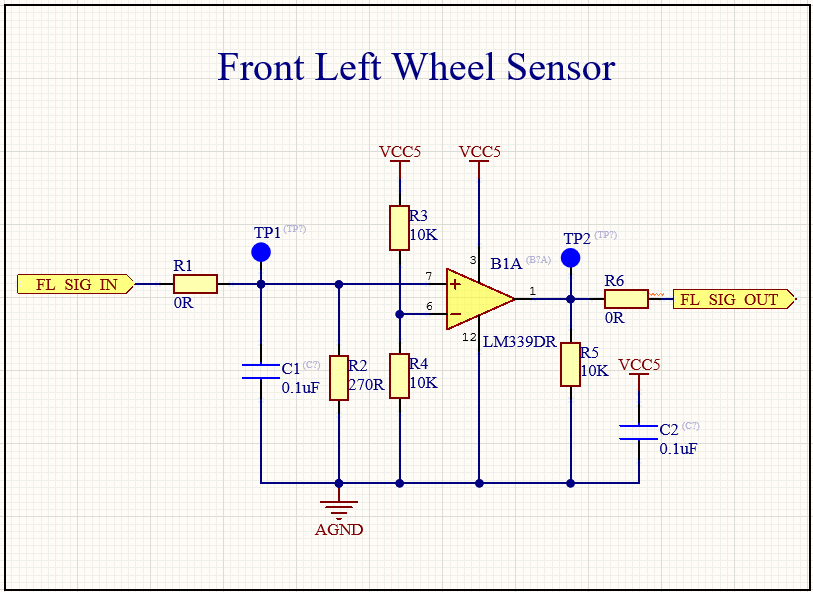
\includegraphics[width=0.8\textwidth]{figuras/circuito-sensor-de-roda-proposto.png}
\end{figure}

O comparador limitado em 2.5V permite transformar o sinal analógico variável em um nível lógico digital, operando em 3.3V para o microcontrolador. A simulação realizada no LTSpice confirma a transição correta entre níveis lógicos conforme as variações do sensor.

\begin{figure}[htbp]
    \centering
    \caption{Simulação do Circuito Sensor de Roda Proposto.}
    \label{fig:ap-simulacao-circuito-sensor-de-roda-proposto}
    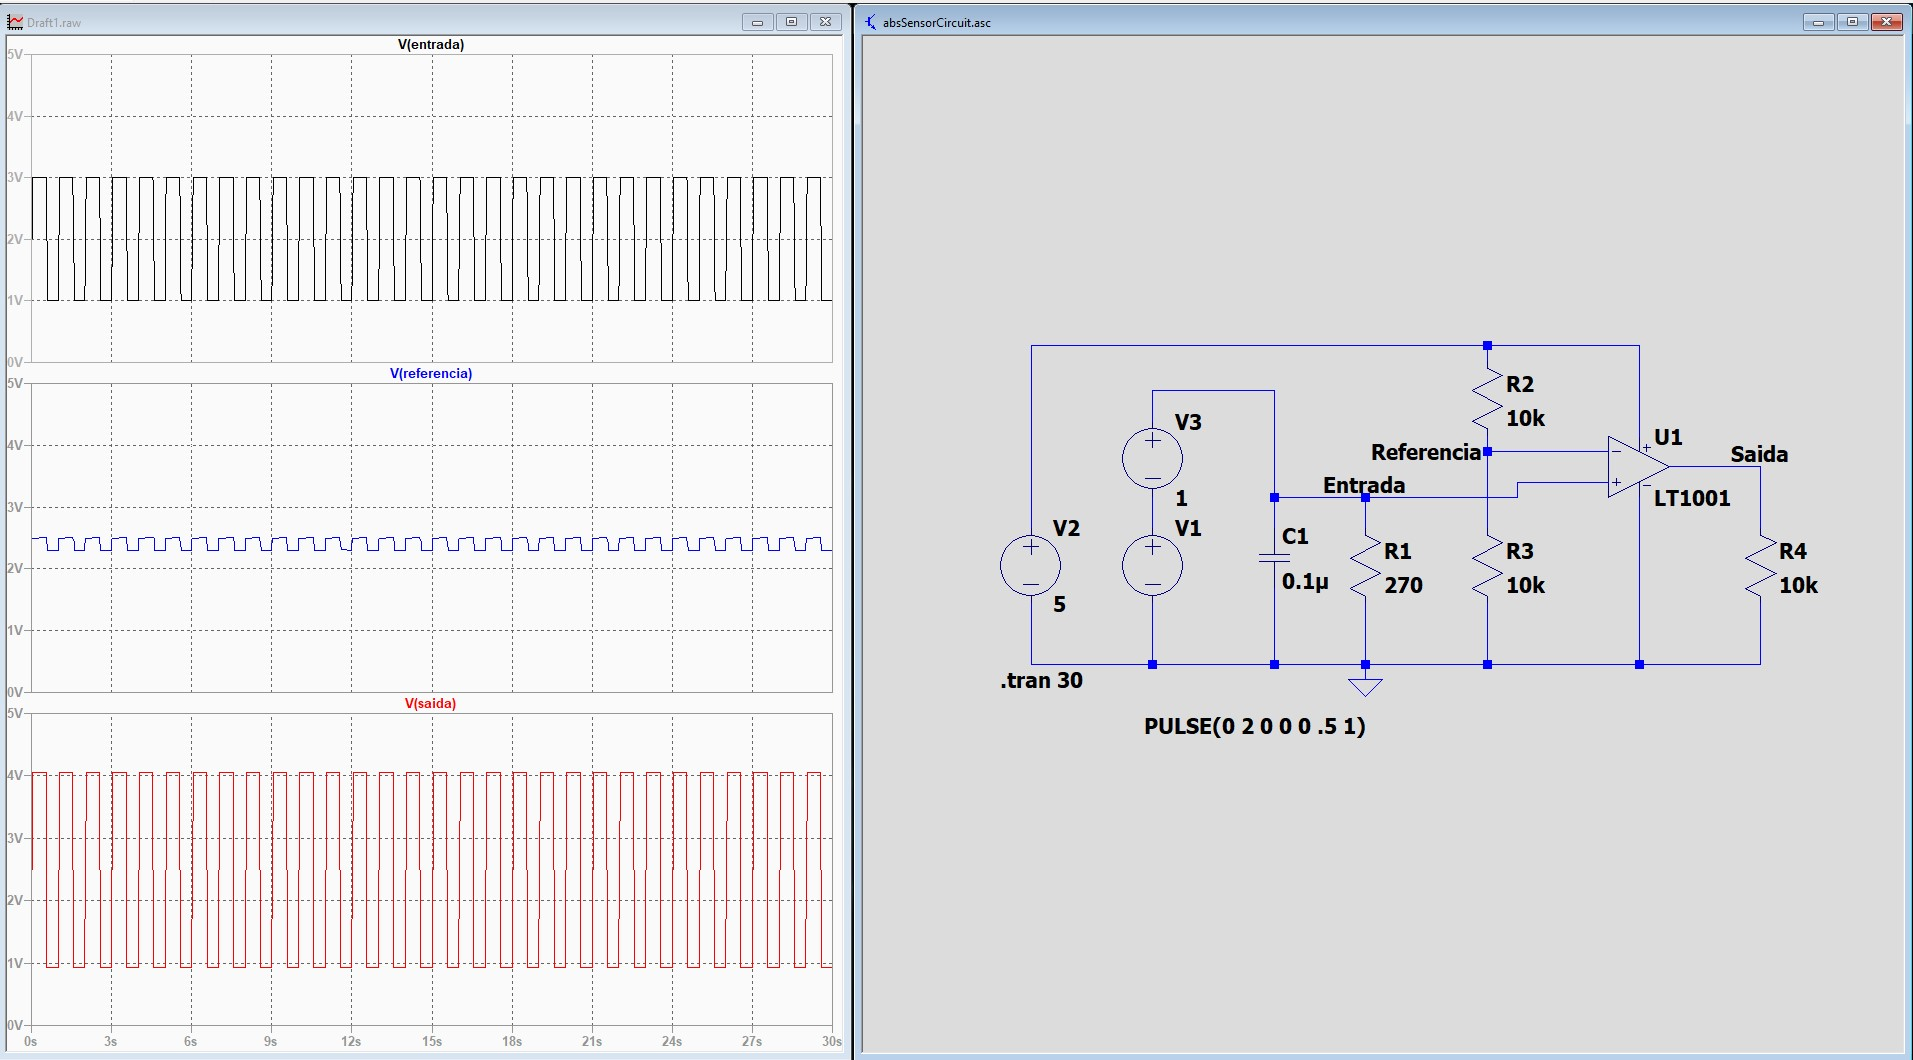
\includegraphics[width=0.8\textwidth]{figuras/simulacao-circuito-sensor-de-roda-proposto.jpg}
\end{figure}

\section{Circuito de Acionamento das Válvulas Solenoides}
\label{ap:circuito-valvulas}

O circuito das válvulas solenoides foi baseado no kit de freio NXP KITVALVECNTLEVM, utilizando os circuitos integrados MC34SB0800 e MC34SB0410, responsáveis pelo controle de múltiplas válvulas e de um motor associado.

\begin{figure}[htbp]
    \centering
    \caption{Circuito de Controle das Válvulas Solenoides.}
    \label{fig:ap-circuito-controle-valvula-solenoide}
    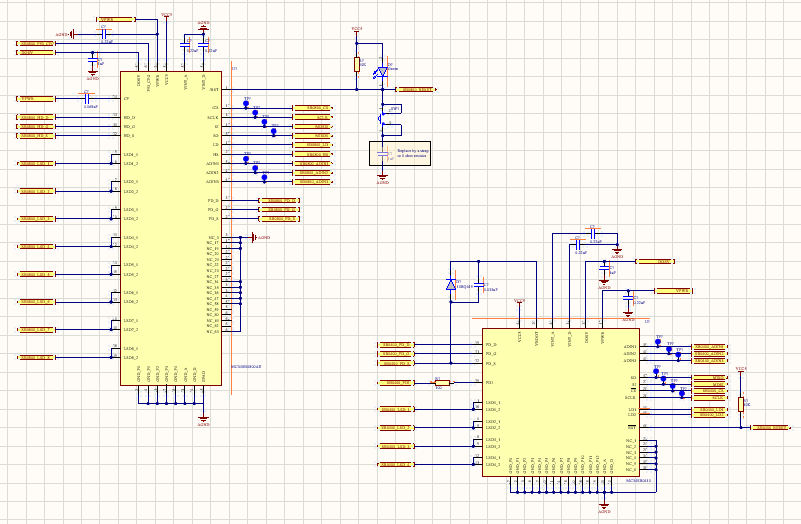
\includegraphics[width=0.8\textwidth]{figuras/circuito-controle-valvula-solenoide.png}
\end{figure}

O uso desses CIs garante proteção de corrente, controle independente das válvulas e compatibilidade com frequências de chaveamento exigidas pela aplicação automotiva.

\section{Circuito de Controle do Motor da Bomba}
\label{ap:circuito-bomba}

Para o acionamento da bomba eletro-hidráulica, o circuito foi desenvolvido com base no mesmo kit da NXP. O MC34SB0800 permite controle \gls{PWM} de até 500 Hz, enquanto o MC34SB0410 opera até 16 kHz, possibilitando controle mais silencioso e preciso.

\begin{figure}[htbp]
    \centering
    \caption{Circuito de Controle da Bomba de Pressão.}
    \label{fig:ap-circuito-controle-bomba}
    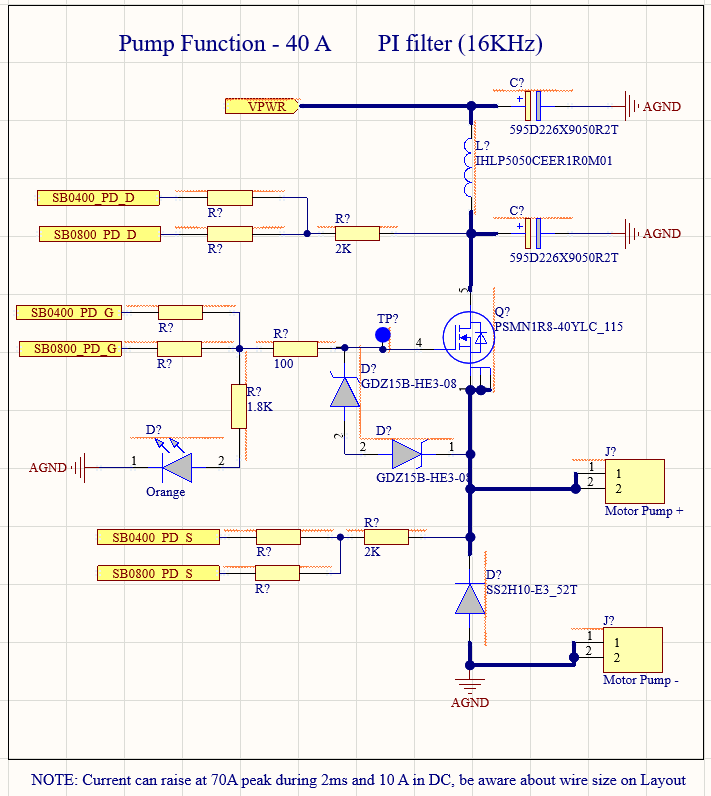
\includegraphics[width=0.8\textwidth]{figuras/circuito-controle-valvula-motor.png}
\end{figure}

Ambos os drivers incluem recursos de proteção e monitoramento essenciais para garantir a integridade do sistema.

\section{Circuito de Leitura do Sensor de Pressão}
\label{ap:circuito-pressao}

Para leitura da pressão hidráulica, selecionou-se um sensor piezoresistivo (strain gauge), devido à robustez e sensibilidade adequada ao sistema de freio. Um amplificador de instrumentação foi utilizado para garantir rejeição de ruído e amplificação precisa do sinal diferencial.

\begin{figure}[htbp]
    \centering
    \caption{Circuito de Leitura do Sensor de Pressão.}
    \label{fig:ap-circuito-sensor-de-pressao}
    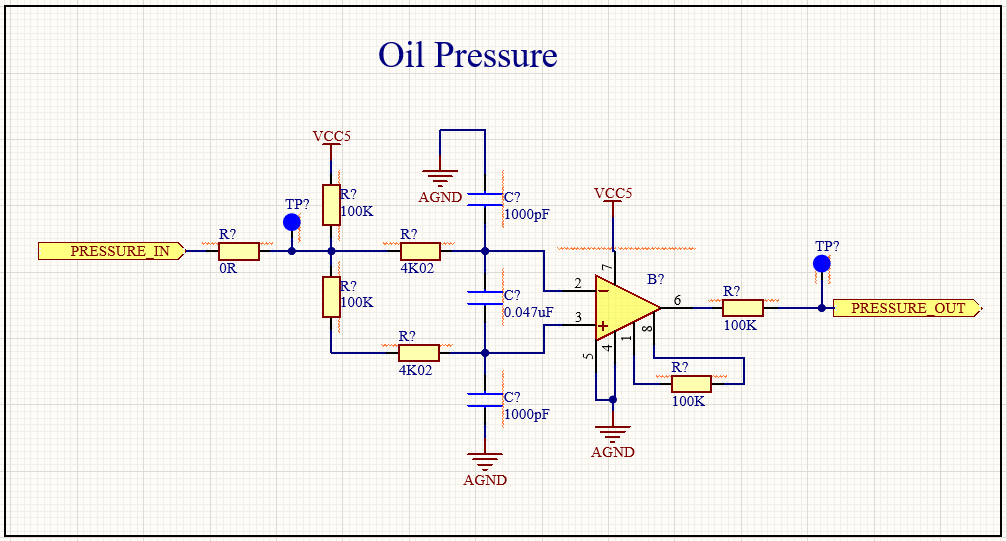
\includegraphics[width=0.8\textwidth]{figuras/circuito-sensor-de-pressao-proposto.png}
\end{figure}

O circuito condiciona o sinal do sensor para níveis adequados de leitura pelo microcontrolador, garantindo estabilidade e confiabilidade durante o processamento dos dados.

\section{Scripts MATLAB e Simulink Utilizados}
\label{ap:scripts-matlab}

Esta seção reúne os scripts utilizados para gerar as figuras de simulação inseridas no trabalho.

Os códigos citados no texto incluem: (i) o bloco \texttt{MATLAB Function} do modelo hidráulico 2P (Código~\ref{cod:bloco_hidraulico_2p}); (ii) o \textit{script} do ensaio integrado em malha aberta (Código~\ref{cod:ensaio_integrado_malha_aberta}); e (iii) o \textit{script} de síntese e execução do controlador LQI (Código~\ref{cod:script_controle_lqi_luenberger}), além dos códigos dos blocos de controle usados no Simulink (Códigos~\ref{cod:matlab_function_lqi_observer} e \ref{cod:matlab_function_valvulas_onoff}).

Inclui-se também o \textit{script} do ensaio integrado em malha aberta na configuração realista, utilizado para gerar a figura \texttt{ensaio\_malha\_aberta\_integrado\_real.png} (Código~\ref{cod:ensaio_integrado_malha_aberta_real}).


\begin{lstlisting}[caption={Bloco MATLAB Function do modelo hidráulico 2P}, label={cod:bloco_hidraulico_2p}, language=Matlab]
function [Psup_dot, Pw_dot, Qpump, Qin, Qout] = Bloco_Hidraulico_2P(omega_p, u_in, u_out, Psup, Pw)
% omega_p: rad/s (>=0)
% u_in, u_out: 0..1 (PWM normalizado / abertura proporcional)
% Psup, Pw: Pa
% Saidas: derivadas de pressao e vazoes (m^3/s)

% ---------- parametros hidraulicos basicos ----------
beta = 1.5e9;   % Pa - modulo volumetrico efetivo (oleo + mangueiras)
rho  = 850;     % kg/m^3 - densidade tipica de fluido de freio
Pret = 1e5;     % Pa - pressao de retorno (aprox. atmosferica)

% ---------- volumes efetivos ----------
Vsup = 6.0e-5;   % m^3
Vw   = 1.0e-5;   % m^3

% ---------- bomba (modelo linear simples) ----------
Dp_rev = 5e-7;                  % m^3/rev
Nv     = 0.85;                  % eficiencia volumetrica
Kb     = Nv * (Dp_rev/(2*pi));  % m^3/rad
Klb    = 6.8e-13;                 % (m^3/s)/Pa

% ---------- valvulas (lei do orificio) ----------
Cv_in    = 0.62;
Cv_out   = 0.62;
Ain_max  = 3.0e-7;              % m^2
Aout_max = 3.0e-7;              % m^2

% Vazamentos opcionais
Kleak_sup = 0;                  % (m^3/s)/Pa
Kleak_w   = 0;                  % (m^3/s)/Pa

% ---------- sanitizacao de entradas ----------
if omega_p < 0
    omega_p = 0;
end
u_in  = min(max(u_in,  0), 1);
u_out = min(max(u_out, 0), 1);

% Evita pressoes abaixo do retorno (numerico)
Psup = max(Psup, Pret);
Pw   = max(Pw,   Pret);

% ---------- bomba -> suprimento ----------
Qpump = Kb*omega_p - Klb*(Psup - Pret);

% ---------- suprimento -> roda (valvula de entrada) ----------
dPin = max(Psup - Pw, 0);
Qin  = Cv_in * (Ain_max * u_in) * sqrt(2*dPin/rho);

% ---------- roda -> retorno (valvula de saida) ----------
dPout = max(Pw - Pret, 0);
Qout  = Cv_out * (Aout_max * u_out) * sqrt(2*dPout/rho);

% ---------- dinamica das pressoes ----------
Psup_dot = (beta/Vsup) * ( Qpump - Qin - Kleak_sup*(Psup - Pret) );
Pw_dot   = (beta/Vw)   * ( Qin - Qout - Kleak_w*(Pw   - Pret) );
end
\end{lstlisting}

\begin{lstlisting}[caption={Script MATLAB do ensaio integrado em malha aberta}, label={cod:ensaio_integrado_malha_aberta}, language=Matlab]
%% ensaio_integrado_malha_aberta.m
% Ensaio integrado em malha aberta:
% Fase A: pressurizacao (omega_p > 0, u_in = 1, u_out = 0)
% Fase B: retencao (omega_p = 0, u_in = 0, u_out = 0)
% Fase C: alivio (omega_p = 0, u_in = 0, u_out > 0)

clear; close all; clc;

mdl = 'BlocoHidraulico';
load_system(mdl);

% Tempo total e condicoes iniciais
Tstop = 4.0;   % s
Pret  = 1e5;   % Pa
Psup0 = Pret;
Pw0   = Pret;
assignin('base','Pret',Pret);
assignin('base','Psup0',Psup0);
assignin('base','Pw0',Pw0);

% Definicao de fases no tempo:
tA_end = 2.0;
tB_end = 3.0;
tC_end = Tstop;

%% Sinal da bomba: omega_p(t)
t_omega = [0    0.5  0.5  1.5  1.5  tA_end ...
           tA_end tB_end tB_end tC_end]';
v_omega = [0    0    30   30   15   15   ...
           0     0    0    0   ]';
omega_p_ts = timeseries(v_omega, t_omega);

%% Sinal da valvula de entrada: u_in(t)
t_uin = [0    tA_end tA_end tC_end]';
v_uin = [1       1      0      0 ]';
u_in_ts = timeseries(v_uin, t_uin);

%% Sinal da valvula de saida: u_out(t)
t_uout = [0    tB_end tB_end tC_end]';
v_uout = [0       0      0.8   0.8 ]';
u_out_ts = timeseries(v_uout, t_uout);

%% Enviar para workspace do modelo
assignin('base','omega_p_ts',omega_p_ts);
assignin('base','u_in_ts',u_in_ts);
assignin('base','u_out_ts',u_out_ts);

%% Configuracao do modelo e simulacao
set_param(mdl, 'StopTime', num2str(Tstop), ...
               'Solver',   'ode15s',      ...
               'MaxStep',  '1e-4');

simOut = sim(mdl);

%% Leitura de sinais (logsout ou To Workspace)
if isprop(simOut,'logsout') && ~isempty(simOut.logsout)
    logs = simOut.logsout;
    getTS = @(name) logs.get(name).Values;
    Psup    = getTS('Psup_bar_g');
    Pw      = getTS('Pw_bar_g');
    Qpump   = getTS('Qpump_mLs');
    Qin     = getTS('Qin_mLs');
    Qout    = getTS('Qout_mLs');
    omega_p = getTS('omega_p');
    u_in    = getTS('u_in');
    u_out   = getTS('u_out');
else
    Psup    = simOut.get('Psup_bar_g');
    Pw      = simOut.get('Pw_bar_g');
    Qpump   = simOut.get('Qpump_mLs');
    Qin     = simOut.get('Qin_mLs');
    Qout    = simOut.get('Qout_mLs');
    omega_p = simOut.get('omega_p');
    u_in    = simOut.get('u_in');
    u_out   = simOut.get('u_out');
end

Psup_g_bar = Psup.Data;
Pw_g_bar   = Pw.Data;
Qpump_ml_s = Qpump.Data;
Qin_ml_s   = Qin.Data;
Qout_ml_s  = Qout.Data;

%% Configuracao de plots
set(groot,'defaultLineLineWidth',1.6);
set(groot,'defaultAxesFontSize',11);
set(groot,'defaultAxesFontName','Times New Roman');

fig = figure('Color','w','Position',[100 100 980 720]);
tiledlayout(3,1,'TileSpacing','compact','Padding','compact');

% Entradas
nexttile;
plot(omega_p.Time, omega_p.Data,'k'); hold on;
plot(u_in.Time,  u_in.Data*max(omega_p.Data),'b--');
plot(u_out.Time, u_out.Data*max(omega_p.Data),'r--');
grid on; ylabel('\\omega_p (rad/s)');
title('Entradas');
legend('\\omega_p','u_{in} (esc.)','u_{out} (esc.)','Location','best');
ymax = max(omega_p.Data); margem = 0.1*ymax;
ylim([-max(2,margem), ymax + max(2,margem)]);
xlim([0 Tstop]);

% Pressoes
nexttile;
plot(Psup.Time, Psup_g_bar,'b'); hold on;
plot(Pw.Time,   Pw_g_bar,'r');
grid on; ylabel('Pressao gauge (bar)'); title('Pressoes');
legend('P_{sup}','P_w','Location','best');
ymin = min([Psup_g_bar(:); Pw_g_bar(:)]);
ymax = max([Psup_g_bar(:); Pw_g_bar(:)]);
ylim([min(ymin,0) ymax + 0.25]);

% Vazoes
nexttile;
plot(Qpump.Time, Qpump_ml_s,'k'); hold on;
plot(Qin.Time,   Qin_ml_s,'b');
plot(Qout.Time,  Qout_ml_s,'r');
grid on; ylabel('Vazao (mL/s)'); xlabel('Tempo (s)');
title('Vazoes');
legend('Q_{pump}','Q_{in}','Q_{out}','Location','best');
ylim([-5 5]);
xlim([0 Tstop]);

%% Exportar figuras
outDir = fullfile(pwd,'figuras');
if ~exist(outDir,'dir'), mkdir(outDir); end
exportgraphics(fig, fullfile(outDir,'ensaio_malha_aberta_integrado.pdf'), 'ContentType','vector');
exportgraphics(fig, fullfile(outDir,'ensaio_malha_aberta_integrado.png'), 'Resolution', 300);
disp('OK: figuras exportadas em:');
disp(outDir);
\end{lstlisting}

\begin{lstlisting}[caption={Script MATLAB do ensaio integrado em malha aberta (configuracao realista)}, label={cod:ensaio_integrado_malha_aberta_real}, language=Matlab]
%% ensaio_integrado_malha_aberta_real.m
% Fases:
% A: pressurizacao (0-2 s): bomba ligada, inlet aberto, outlet fechado
% B: retencao (2-3 s): bomba desligada, valvulas fechadas
% C: alivio (3-4 s): bomba desligada, inlet fechado, outlet parcialmente aberto

clear; close all; clc;

mdl = 'BlocoHidraulico';   % modelo Simulink que chama Bloco_Hidraulico_2P
load_system(mdl);

% Tempo total e condicoes iniciais
Tstop = 4.0;   % s
Pret  = 1e5;   % Pa
Psup0 = Pret;
Pw0   = Pret;
assignin('base','Pret',Pret);
assignin('base','Psup0',Psup0);
assignin('base','Pw0',Pw0);

% Fases
tA_end = 2.0;
tB_end = 3.0;
tC_end = Tstop;

%% Sinal da bomba: omega_p(t)
% Valores de referencia:
t_omega = [0   0.05 0.05  0.5  0.5  tA_end ...
           tA_end tB_end tB_end tC_end]';
v_omega = [0   0    100   100  100  100  ...
           0     0    0    0   ]';  % 100 rad/s aprox. 1000 rpm
omega_p_ts = timeseries(v_omega, t_omega);

%% Sinal da valvula de entrada: u_in(t)
% Fase A: aberta; Fases B e C: fechada.
t_uin = [0    tA_end tA_end tC_end]';
v_uin = [1       1      0      0 ]';
u_in_ts = timeseries(v_uin, t_uin);

%% Sinal da valvula de saida: u_out(t)
% Fases A e B: fechada; Fase C: 80% aberta.
t_uout = [0    tB_end tB_end tC_end]';
v_uout = [0       0      0.8   0.8 ]';
u_out_ts = timeseries(v_uout, t_uout);

%% Enviar sinais para o workspace do modelo
assignin('base','omega_p_ts',omega_p_ts);
assignin('base','u_in_ts',u_in_ts);
assignin('base','u_out_ts',u_out_ts);

%% Configuracao do modelo e simulacao
set_param(mdl, 'StopTime', num2str(Tstop), ...
               'Solver',   'ode15s',      ...
               'MaxStep',  '1e-4');

simOut = sim(mdl);

%% Leitura de sinais
if isprop(simOut,'logsout') && ~isempty(simOut.logsout)
    logs = simOut.logsout;
    getTS = @(name) logs.get(name).Values;
    Psup    = getTS('Psup_bar_g');
    Pw      = getTS('Pw_bar_g');
    Qpump   = getTS('Qpump_mLs');
    Qin     = getTS('Qin_mLs');
    Qout    = getTS('Qout_mLs');
    omega_p = getTS('omega_p');
    u_in    = getTS('u_in');
    u_out   = getTS('u_out');
else
    Psup    = simOut.get('Psup_bar_g');
    Pw      = simOut.get('Pw_bar_g');
    Qpump   = simOut.get('Qpump_mLs');
    Qin     = simOut.get('Qin_mLs');
    Qout    = simOut.get('Qout_mLs');
    omega_p = simOut.get('omega_p');
    u_in    = simOut.get('u_in');
    u_out   = simOut.get('u_out');
end

Psup_g_bar = Psup.Data;   % bar (gauge)
Pw_g_bar   = Pw.Data;     % bar (gauge)
Qpump_ml_s = Qpump.Data;  % mL/s
Qin_ml_s   = Qin.Data;
Qout_ml_s  = Qout.Data;

%% Configuracao de plots
set(groot,'defaultLineLineWidth',1.6);
set(groot,'defaultAxesFontSize',11);
set(groot,'defaultAxesFontName','Times New Roman');

fig = figure('Color','w','Position',[100 100 980 720]);
tiledlayout(3,1,'TileSpacing','compact','Padding','compact');

% Entradas
nexttile;
plot(omega_p.Time, omega_p.Data,'k'); hold on;
plot(u_in.Time,  u_in.Data*max(omega_p.Data),'b--');
plot(u_out.Time, u_out.Data*max(omega_p.Data),'r--');
grid on; ylabel('\\omega_p (rad/s)');
title('Entradas');
legend('\\omega_p','u_{in} (esc.)','u_{out} (esc.)','Location','best');
ymax = max(omega_p.Data); margem = 0.1*ymax;
ylim([-max(2,margem), ymax + max(2,margem)]);
xlim([0 Tstop]);

% Pressoes
nexttile;
plot(Psup.Time, Psup_g_bar,'b'); hold on;
plot(Pw.Time,   Pw_g_bar,'r');
grid on; ylabel('Pressao gauge (bar)'); title('Pressoes');
legend('P_{sup}','P_w','Location','best');
ymin = min([Psup_g_bar(:); Pw_g_bar(:)]);
ymax = max([Psup_g_bar(:); Pw_g_bar(:)]);
ylim([min(ymin,0) ymax + 5]);
xlim([0 Tstop]);

% Vazoes
nexttile;
plot(Qpump.Time, Qpump_ml_s,'k'); hold on;
plot(Qin.Time,   Qin_ml_s,'b');
plot(Qout.Time,  Qout_ml_s,'r');
grid on; ylabel('Vazao (mL/s)'); xlabel('Tempo (s)');
title('Vazoes');
legend('Q_{pump}','Q_{in}','Q_{out}','Location','best');
ylim([-60 60]);
xlim([0 Tstop]);

%% Exportar figuras
outDir = fullfile(pwd,'figuras');
if ~exist(outDir,'dir'), mkdir(outDir); end
exportgraphics(fig, fullfile(outDir,'ensaio_malha_aberta_integrado_real.pdf'), 'ContentType','vector');
exportgraphics(fig, fullfile(outDir,'ensaio_malha_aberta_integrado_real.png'), 'Resolution', 300);
disp('OK: figuras exportadas em:');
disp(outDir);
\end{lstlisting}

\begin{lstlisting}[caption={Script MATLAB do projeto do controle LQI discreto (baseado em linearização local) e execução do modelo Simulink}, label={cod:script_controle_lqi_luenberger}, language=Matlab]
%% ============================================================
% CONTROLE LQR DISCRETO + OBSERVADOR DE LUENBERGER
% SISTEMA HIDRÁULICO DE FREIO NÃO LINEAR
% =============================================================

clear; clc; close all;

%% =============================================================
% 1) PARÂMETROS FÍSICOS (iguais ao modelo não linear)
% =============================================================
beta = 1.5e9;
rho  = 850;
Pret = 1e5;

Vsup = 6.0e-5;
Vw   = 1.0e-5;

Dp_rev = 5e-7;
Nv     = 0.85;
Kb     = Nv * (Dp_rev/(2*pi));
Klb    = 6.8e-13; % ATENCAO: manter consistente com o modelo nao linear (planta)

Cv_in   = 0.62;
Cv_out  = 0.62;
Ain_max = 3.0e-7;
Aout_max= 3.0e-7;

%% =============================================================
% 2) PONTO DE OPERAÇÃO
% =============================================================
Pw_op   = Pret + 100e5;        % Pa (100 bar gauge)
Psup_op = Pw_op + 5e5;         % Pa (5 bar de diferencial na valvula de entrada)

u_in_op  = 0.5;
u_out_op = 0.0;

% vazão necessária para manter equilíbrio
dPin = Psup_op - Pw_op;
Qin_op = Cv_in*(Ain_max*u_in_op)*sqrt(2*dPin/rho);

omega_op = Qin_op / Kb;

%% =============================================================
% 3) LINEARIZAÇÃO ANALÍTICA
% Estados: x = [Psup Pw]'
% Entrada: u = omega_p
% Saída: y = Pw
% =============================================================

% Qin = kq*sqrt(2*(Psup-Pw)/rho), com kq = Cv_in*Ain_max*u_in_op
kq  = Cv_in*Ain_max*u_in_op;
s   = sqrt(2*dPin/rho);
dQd = kq/(rho*s); % dQin/d(Psup-Pw)

% Psup_dot = (beta/Vsup)*(Kb*omega_p - Klb*(Psup-Pret) - Qin)
% Pw_dot   = (beta/Vw)  *(Qin)  (com u_out_op=0 no ponto)
a11 = -(beta/Vsup)*(Klb + dQd);
a12 =  (beta/Vsup)*(dQd);

a21 =  (beta/Vw)*(dQd);
a22 = -(beta/Vw)*(dQd);

A = [a11 a12;
     a21 a22];

B = [(beta/Vsup)*Kb;
      0];

C = [0 1];
D = 0;

sys_c = ss(A,B,C,D);

%% =============================================================
% 4) PROJETO LQR CONTÍNUO
% =============================================================
Q = diag([1e-12 1e-10]);
R = 1e-6;

K = lqr(A,B,Q,R);

%% =============================================================
% 5) OBSERVADOR DE LUENBERGER
% =============================================================
desired_poles = 5*eig(A);
L = place(A',C',desired_poles)';

%% ============================================================
% PROJETO LQI DISCRETO
% =============================================================

Ts = 1e-4;

sys_d = c2d(sys_c,Ts);

Ad = sys_d.A;
Bd = sys_d.B;
Cd = sys_d.C;

%% Sistema aumentado para LQI
Ad_aug = [Ad zeros(2,1);
         -Cd*Ts 1];

Bd_aug = [Bd; 0];

Q_aug = diag([1e-12 1e-10 1e4]);
R = 1e-7;

K_aug = dlqr(Ad_aug,Bd_aug,Q_aug,R);

Kx = K_aug(1:2);
Ki = K_aug(3);

%% Observador discreto
Ld = place(Ad',Cd',0.4*eig(Ad))';

assignin('base','Ad',Ad);
assignin('base','Bd',Bd);
assignin('base','Cd',Cd);
assignin('base','Kx',Kx);
assignin('base','Ki',Ki);
assignin('base','Ld',Ld);
assignin('base','Ts',Ts);
assignin('base','Kb',Kb);
assignin('base','Klb',Klb);
assignin('base','Pret',Pret);


%% ============================================================
% EXECUÇÃO DO CONTROLADOR - Freio_LQR_Model
% =============================================================

%% Tempo de simulação
Ts = 1e-4;
Tf = 3;
t  = (0:Ts:Tf)';

%% =============================================================
% SINAL DE REFERÊNCIA: 0-50-30-80-20-100 (bar)
% =============================================================

Pref_bar = zeros(size(t));

Pref_bar(t>=0.5) = 50;
Pref_bar(t>=1.0) = 30;
Pref_bar(t>=1.5) = 80;
Pref_bar(t>=2.0) = 20;
Pref_bar(t>=2.5) = 100;

Pref = Pref_bar * 1e5;   % converter para Pa

%% Entrada do controlador
Pref_ts = timeseries(Pref,t);

assignin('base','Pref_ts',Pref_ts);

%% ============================================================
% Configurar modelo
% =============================================================

model = 'Freio_LQR_Model';

set_param(model,'Solver','FixedStepDiscrete');
set_param(model,'FixedStep',num2str(Ts));
set_param(model,'StopTime',num2str(Tf));

%% ============================================================
% Rodar simulação
% =============================================================

simOut = sim(model);

%% ============================================================
% Captura dos sinais direto do Simulink (logsout)
% =============================================================

% Rodar simulação
simOut = sim('Freio_LQR_Model');

% Extrair sinais usando logsout
logs = simOut.logsout;

getTS = @(name) logs.get(name).Values; % função para extrair timeseries

omega_p = getTS('omega_p');    % comando do motor
u_in    = getTS('u_in');       % válvula entrada
u_out   = getTS('u_out');      % válvula saída
Psup    = getTS('Psup_bar');   % pressão sup
Pw      = getTS('Pw_bar');     % pressão Pw
Pref    = getTS('Pref_bar');   % referência de pressão

Tstop = max(Psup.Time);        % tempo final da simulação

%% ============================================================
% Configuração de plots
% =============================================================

set(groot,'defaultLineLineWidth',1.6);
set(groot,'defaultAxesFontSize',11);
set(groot,'defaultAxesFontName','Times New Roman');

fig = figure('Color','w','Position',[100 100 980 720]);
tiledlayout(3,1,'TileSpacing','compact','Padding','compact');

% 1) Entradas / Comandos
nexttile;
plot(omega_p.Time, squeeze(omega_p.Data),'k'); hold on;
plot(u_in.Time,  squeeze(u_in.Data)*max(squeeze(omega_p.Data)),'b--');
plot(u_out.Time, squeeze(u_out.Data)*max(squeeze(omega_p.Data)),'r--');
grid on; ylabel('\\omega_p (rad/s)');
title('Sinais de comando');
legend('\\omega_p','u_{in} (esc.)','u_{out} (esc.)','Location','best');
ylim([-0.1*max(squeeze(omega_p.Data)), 1.1*max(squeeze(omega_p.Data))]);
xlim([0 Tstop]);

% 2) Pressões
nexttile;
plot(Psup.Time, squeeze(Psup.Data),'b'); hold on;
plot(Pw.Time,   squeeze(Pw.Data),'r');
plot(Pref.Time, squeeze(Pref.Data),'k--');
grid on; ylabel('Pressão (bar)'); title('Pressões e referência');
legend('P_{sup}','P_w','Pref','Location','best');
ymin = min([squeeze(Psup.Data); squeeze(Pw.Data); squeeze(Pref.Data)]);
ymax = max([squeeze(Psup.Data); squeeze(Pw.Data); squeeze(Pref.Data)]);
ylim([ymin-5, ymax+5]);
xlim([0 Tstop]);

%% ============================================================
% Exportar figuras
% =============================================================

outDir = fullfile(pwd,'figuras');
if ~exist(outDir,'dir'), mkdir(outDir); end

exportgraphics(fig, fullfile(outDir,'simulacao_comandos_e_pressao.pdf'), 'ContentType','vector');
exportgraphics(fig, fullfile(outDir,'simulacao_comandos_e_pressao.png'), 'Resolution', 300);

disp('OK: figuras exportadas em:');
disp(outDir);

%% ============================================================
% MÉTRICAS DE DESEMPENHO (r(t) em patamares)
% Gera uma figura com resumo: e_RMS, Mp, tr, ts, e_inf e esforços máximos.
% ============================================================

% Dados em bar (conforme logsout)
t = Pref.Time;
r = squeeze(Pref.Data);
y = squeeze(Pw.Data);

e = r - y;

% RMS do erro (bar)
Ttotal = t(end) - t(1);
e_rms = sqrt(trapz(t, e.^2) / max(Ttotal, eps));

% Esforço máximo (atuadores)
omega_max = max(squeeze(omega_p.Data));
u_in_max  = max(squeeze(u_in.Data));
u_out_max = max(squeeze(u_out.Data));

% Identifica degraus na referência
idx_steps = find(diff(r) ~= 0) + 1;
idx_steps = idx_steps(:);
idx_all = [idx_steps; numel(t)+1];

% Parâmetros para métricas por degrau
alpha_rise = [0.1 0.9];  % 10%-90%
tol_frac   = 0.02;       % 2% de banda de acomodação

% Estruturas para relatório
lines = {};
lines{end+1} = sprintf('e_{RMS} = %.3f bar', e_rms);
lines{end+1} = sprintf('max(\\omega_p) = %.1f rad/s', omega_max);
lines{end+1} = sprintf('max(u_{in}) = %.2f, max(u_{out}) = %.2f', u_in_max, u_out_max);

for k = 1:numel(idx_steps)
    i0 = idx_steps(k);
    i1 = idx_all(k+1) - 1;
    if i1 <= i0, continue; end

    t0 = t(i0);
    r0 = r(i0-1);
    r1 = r(i0);
    y0 = y(i0-1);

    dt = r1 - r0;
    if abs(dt) < 1e-9, continue; end

    ts = t(i0:i1);
    ys = y(i0:i1);

    % Overshoot (Mp) em % do degrau
    if dt > 0
        peak = max(ys);
        Mp = 100 * max(0, peak - r1) / abs(dt);
    else
        peak = min(ys);
        Mp = 100 * max(0, r1 - peak) / abs(dt);
    end

    % Rise time (10%-90%)
    y10 = y0 + alpha_rise(1)*dt;
    y90 = y0 + alpha_rise(2)*dt;

    if dt > 0
        i10 = find(ys >= y10, 1, 'first');
        i90 = find(ys >= y90, 1, 'first');
    else
        i10 = find(ys <= y10, 1, 'first');
        i90 = find(ys <= y90, 1, 'first');
    end

    if isempty(i10) || isempty(i90)
        tr = NaN;
    else
        tr = ts(i90) - ts(i10);
    end

    % Settling time (2% da amplitude do degrau)
    band = tol_frac * abs(dt);
    outside = find(abs(ys - r1) > band);
    if isempty(outside)
        ts_settle = 0;
    else
        last_out = outside(end);
        if last_out == numel(ts)
            ts_settle = NaN;
        else
            ts_settle = ts(last_out) - t0;
        end
    end

    % Erro estacionário: média do último 10% do segmento
    n_tail = max(5, round(0.1*numel(ts)));
    e_inf = mean((r(i1-n_tail+1:i1) - y(i1-n_tail+1:i1)));

    lines{end+1} = sprintf('Degrau @ t=%.2fs: r %.0f->%.0f bar | Mp=%.1f%% | tr=%.3fs | ts=%.3fs | e_inf=%.3f bar', ...
        t0, r0, r1, Mp, tr, ts_settle, e_inf);
end

% Figura de métricas
figm = figure('Color','w','Position',[100 100 1100 700]);
tiledlayout(2,1,'TileSpacing','compact','Padding','compact');

nexttile;
plot(t, y,'r','LineWidth',1.4); hold on;
plot(t, r,'k--','LineWidth',1.2);
grid on;
ylabel('Pressão (bar)');
title('Resposta e referência (Pw)');
legend('P_w','P_{ref}','Location','best');

nexttile;
plot(t, e,'b','LineWidth',1.2);
grid on;
ylabel('Erro (bar)'); xlabel('Tempo (s)');
title('Erro de seguimento e(t) = r(t) - y(t)');

% Caixa de texto com resumo
txt = strjoin(lines, '\n');
annotation(figm,'textbox',[0.04 0.02 0.92 0.26], ...
    'String',txt,'FitBoxToText','off','Interpreter','tex', ...
    'EdgeColor',[0.2 0.2 0.2],'BackgroundColor',[1 1 1]);

exportgraphics(figm, fullfile(outDir,'metricas_desempenho.pdf'), 'ContentType','vector');
exportgraphics(figm, fullfile(outDir,'metricas_desempenho.png'), 'Resolution', 300);

disp('OK: figura de métricas exportada em:');
disp(outDir);
\end{lstlisting}

\begin{lstlisting}[caption={Bloco \texttt{MATLAB Function}: controlador discreto (LQI) com observador de Luenberger para gerar $\omega_p$}, label={cod:matlab_function_lqi_observer}, language=Matlab]
function omega_p = LQI_Observer(Pw, Pref)

%#codegen

Ad = coder.const(Ad);
Bd = coder.const(Bd);
Cd = coder.const(Cd);
Kx = coder.const(Kx);
Ki = coder.const(Ki);
Ld = coder.const(Ld);
Ts = coder.const(Ts);
Kb = coder.const(Kb);
Klb = coder.const(Klb);
Pret = coder.const(Pret);

persistent xhat xi u_prev

if isempty(xhat)
    xhat = zeros(2,1);
end

if isempty(xi)
    xi = 0;
end

if isempty(u_prev)
    u_prev = 0;
end

% ===== Observador discreto =====
% Nota: em implementação real, u_prev representa o comando aplicado no passo anterior.
xhat = Ad*xhat + Bd*u_prev + Ld*(Pw - Cd*xhat);

% ===== Seguimento + anti-windup =====
% Erro em Pa (entrada do modelo em Pa)
erro = Pref - Pw;

% Limite fisico coerente com pressao maxima de suprimento
% (P_sup,max - P_ret) ~= Kb*omega_p_max/Klb  =>  omega_p_max ~= (P_sup,max-Pret)*Klb/Kb
P_sup_max_bar = 130; % bar (gauge) - ajustar conforme alvo fisico
P_sup_max = Pret + P_sup_max_bar*1e5;
omega_p_max = (P_sup_max - Pret) * (Klb / max(Kb, eps));

% Integracao candidata
xi_cand = xi + erro*Ts;

% Lei LQI (nao saturada)
omega_unsat = -Kx*xhat - Ki*xi_cand;

% Saturacao (bomba nao reversivel: omega>=0)
omega_sat = omega_unsat;
if omega_sat < 0
    omega_sat = 0;
end
if omega_sat > omega_p_max
    omega_sat = omega_p_max;
end

% Anti-windup por integracao condicional:
% se saturou e o erro empurra na mesma direcao da saturacao, congela integrador
is_saturated = (omega_sat ~= omega_unsat);
if is_saturated
    if (omega_sat <= 0 && erro < 0) || (omega_sat >= omega_p_max && erro > 0)
        % mantem xi
    else
        xi = xi_cand;
    end
else
    xi = xi_cand;
end

omega_p = omega_sat;

u_prev = omega_p;

end
\end{lstlisting}

\begin{lstlisting}[caption={Bloco \texttt{MATLAB Function}: lógica discreta (on/off com histerese) para válvulas de entrada e saída}, label={cod:matlab_function_valvulas_onoff}, language=Matlab]
function [u_in,u_out] = Valvulas_ONOFF(Pw,Pref)

%#codegen

delta_on  = 2e5;  % 2 bar
delta_off = 1e5;  % 1 bar

persistent state
%  1 = enchendo
%  0 = neutro
% -1 = esvaziando

if isempty(state)
    state = 0;
end

erro = Pref - Pw;

switch state
    case 0
        if erro > delta_on
            state = 1;
        elseif erro < -delta_on
            state = -1;
        end
    case 1
        if erro < delta_off
            state = 0;
        end
    case -1
        if erro > -delta_off
            state = 0;
        end
end

u_in  = double(state == 1);
u_out = double(state == -1);

end
\end{lstlisting}

\section{Ponto de operação utilizado na linearização}
\label{ap:ponto-operacao}

Esta seção reúne os valores numéricos adotados como ponto de operação $(x_0,u_0)$ no processo de linearização local do modelo hidráulico. O ponto é escolhido em regime de frenagem, satisfazendo $P_{sup,0}>P_{w,0}>P_{ret}$, de modo a manter $\Delta P>0$ nas leis de vazão e evitar indeterminações nas raízes quadradas.

Os valores utilizados no script de projeto do controle (Código~\ref{cod:script_controle_lqi_luenberger}) são apresentados na Tabela~\ref{tab:ponto_operacao_linearizacao}.

\begin{table}[htbp]
    \Caption{\label{tab:ponto_operacao_linearizacao} Ponto de operação $(x_0,u_0)$ adotado na linearização local}
    \UNIFORtab{}{
        \begin{tabular}{l|l|l}
            \hline
            Grandeza                                     & Símbolo           & Valor adotado                                            \\
            \hline
            Pressão de retorno                           & $P_{ret}$         & $1{,}0\times 10^{5}\,\text{Pa}$ (1 bar)                  \\
            Pressão no canal/roda                        & $P_{w,0}$         & $1{,}01\times 10^{7}\,\text{Pa}$ ($\approx$101 bar abs.) \\
            Pressão no suprimento/manifold               & $P_{sup,0}$       & $1{,}06\times 10^{7}\,\text{Pa}$ ($\approx$106 bar abs.) \\
            Comando nominal válvula de entrada           & $u_{in,0}$        & 0{,}5                                                    \\
            Comando nominal válvula de saída             & $u_{out,0}$       & 0{,}0                                                    \\
            Diferencial de pressão na válvula de entrada & $\Delta P_{in,0}$ & $5{,}0\times 10^{5}\,\text{Pa}$ (5 bar)                  \\
            Vazão nominal pela válvula de entrada        & $Q_{in,0}$        & $\approx 3{,}19\times 10^{-6}\,\text{m}^3/\text{s}$      \\
            Velocidade nominal da bomba (equilíbrio)     & $\omega_{p,0}$    & $\approx 47{,}2\,\text{rad/s}$                           \\
            \hline
        \end{tabular}
    }{\Fonte{Valores calculados a partir do script MATLAB apresentado no Código~\ref{cod:script_controle_lqi_luenberger}.}}
\end{table}

\section{Matrizes linearizadas (A, B, C, D)}
\label{ap:matrizes-lin}

Esta seção apresenta as matrizes obtidas no ponto de operação da Tabela~\ref{tab:ponto_operacao_linearizacao}, conforme o procedimento implementado no Código~\ref{cod:script_controle_lqi_luenberger}. Considera-se o modelo contínuo linearizado com estados $x=[P_{sup}\ \ P_w]^\top$, entrada $u=\omega_p$ e saída $y=P_w$.

As matrizes contínuas $(A,B,C,D)$ são:
\begin{equation}
    A =
    \begin{bmatrix}
        -3{,}30\times 10^{2}           & \phantom{-}7{,}97\times 10^{1} \\
        \phantom{-}4{,}78\times 10^{2} & -4{,}78\times 10^{2}
    \end{bmatrix},
    \qquad
    B =
    \begin{bmatrix}
        1{,}69\times 10^{6} \\
        0
    \end{bmatrix},
    \qquad
    C =
    \begin{bmatrix}
        0 & 1
    \end{bmatrix},
    \qquad
    D = 0.
\end{equation}

No projeto digital, as matrizes discretas $(A_d,B_d,C_d)$ são obtidas por retenção de ordem zero (ZOH) com $T_s=10^{-4}$~s via \texttt{c2d}, conforme o Código~\ref{cod:script_controle_lqi_luenberger}.


\chapter{Códigos MATLAB utilizados nas simulações}
\label{ap:codigos-matlab}

Este apêndice reúne rotinas auxiliares utilizadas para parametrizar ensaios e gerar sinais de referência no ambiente MATLAB/Simulink. Os trechos são apresentados para fins de reprodutibilidade do procedimento.

\section{Mapeamento simples de desaceleração para referência de pressão}
\label{ap:codigos-matlab-mapeamento}

A Listagem~\ref{lst:accel-to-pressure} mostra a função empregada para gerar um perfil de referência de pressão $P_{\mathrm{ref}}$ a partir de uma desaceleração desejada $a_{\mathrm{ego}}(t)$. Por construção, o mapeamento aplica pressão apenas quando $a_{\mathrm{ego}}(t)\le 0$.

\begin{lstlisting}[language=Matlab,caption={Funcao para converter desaceleracao em referencia de pressao.},label={lst:accel-to-pressure}]
function Pref = accel_to_pressure(a_ego)
m  = 1500;          % mass [kg]
Ac = 2e-3;          % equivalent area [m^2]
a  = min(a_ego, 0); % braking only (negative)
F  = m * abs(a);    % braking force [N]
Pref = F / Ac;      % required pressure [Pa]
end
\end{lstlisting}

\chapter{Trechos selecionados do firmware em C}
\label{ap:codigo-c-firmware}

Os excertos de código apresentados nesta seção documentam a estrutura algorítmica implementada no microcontrolador AURIX TC375 para os ensaios em bancada. A rotina do Código~\ref{cod:c-ppmulti-lqi} detalha a realização discreta do controle em cascata empregado no ensaio \texttt{PPMULTI} (Figura~\ref{fig:resultado-final-ppmulti}), explicitando a sincronização do observador de Luenberger, os limites de saturação e a composição das ações de controle de posição e pressão. As métricas quantitativas de desempenho em regime de múltiplos patamares são tratadas de forma dedicada na Tabela~\ref{tab:resultado-final-clmulti-metricas} para a configuração \texttt{CLMULTI}.

Este capítulo apresenta excertos do firmware em C relacionados aos ensaios experimentais discutidos no Capítulo~\ref{chap:resultados-final}. Foram mantidos somente trechos necessários para documentar o acionamento, o processamento de sinais e o registro de dados.

\section{Aquisição e registro dos ensaios em bancada}
\label{ap:codigo-c-aquisicao}

No ensaio \texttt{OLTEST}, o firmware calcula os comandos em malha aberta, consulta as telemetrias hidráulica e mecânica e envia, em intervalos regulares, uma linha com tempo, comandos, pressão, posição, estado e modo das válvulas. O formato de registro associado à Figura~\ref{fig:resultado-final-oltest} é exemplificado no Código~\ref{cod:c-oltest-telemetria}.

\begin{lstlisting}[language=C,caption={Registro serial de telemetria do ensaio OLTEST.},label={cod:c-oltest-telemetria}]
g_olLogCounterMs++;
if (g_olLogCounterMs >= BRAKE_OL_LOG_PERIOD_MS)
{
    BrakeHydraulics_Mode valveMode;
    g_olLogCounterMs = 0u;
    BrakeHydraulics_GetMode(&valveMode);
    BrakeUartTest_Printf("[OL],%lu,%.2f,%u,%u,%.2f,%.2f,%u,%u\r\n",
                         (unsigned long)g_olElapsedMs,
                         posMm,
                         (unsigned int)uIn,
                         (unsigned int)uOut,
                         pwPsi,
                         hydraulicTelemetry.pistonPositionMm,
                         (unsigned int)hydraulicTelemetry.status,
                         (unsigned int)valveMode);
}
\end{lstlisting}

O ensaio \texttt{PLID} identifica a posição no instante em que cada referência de pressão é atingida e calcula médias durante a retenção. O trecho do Código~\ref{cod:c-plid-retencao} corresponde ao processamento que fundamenta a análise da Figura~\ref{fig:resultado-final-plid}.

\begin{lstlisting}[language=C,caption={Deteccao de referencia e calculo das medias de retencao no ensaio PLID.},label={cod:c-plid-retencao}]
case BrakeUartTest_Plid_Pressurize:
    if (pwReal >= g_plidTargetPsi[g_plidStepIndex])
    {
        MotorPlatform_Stop();
        g_plidPosAtTarget[g_plidStepIndex] = posReal;
        (void)BrakeHydraulics_SetMode(
            BrakeHydraulics_ModeHoldCandidate);
        g_plidPhase = BrakeUartTest_Plid_Hold;
        g_plidPhaseMs = 0u;
    }
    break;

case BrakeUartTest_Plid_Hold:
    (void)BrakeHydraulics_SetMode(
        BrakeHydraulics_ModeHoldCandidate);
    g_plidPwAtHold[g_plidStepIndex] += pwReal;
    g_plidPosAtHold[g_plidStepIndex] += posReal;
    g_plidHoldSamples[g_plidStepIndex]++;

    if (g_plidPhaseMs >= BRAKE_PLID_T_HOLD_MS)
    {
        if (g_plidHoldSamples[g_plidStepIndex] > 0u)
        {
            g_plidPwAtHold[g_plidStepIndex] /=
                (float)g_plidHoldSamples[g_plidStepIndex];
            g_plidPosAtHold[g_plidStepIndex] /=
                (float)g_plidHoldSamples[g_plidStepIndex];
        }
        BrakeUartTest_Printf(
            "[PLID] Hold: Pw_med=%.1f pos_med=%.2f\r\n",
            g_plidPwAtHold[g_plidStepIndex],
            g_plidPosAtHold[g_plidStepIndex]);
        MotorPlatform_Stop();
        (void)BrakeHydraulics_SetMode(
            BrakeHydraulics_ModeReleaseValidated);
        g_plidPhase = BrakeUartTest_Plid_Release;
        g_plidPhaseMs = 0u;
    }
    break;
\end{lstlisting}

Para o ensaio \texttt{STAIRCASE}, o firmware registra a referência de posição, a posição medida e a pressão filtrada em cada amostra exportada. Esse registro permite relacionar a curva experimental da Figura~\ref{fig:resultado-final-staircase} ao movimento do atuador e à telemetria hidráulica, conforme o Código~\ref{cod:c-staircase-telemetria}.

\begin{lstlisting}[language=C,caption={Registro de posicao e pressao no ensaio STAIRCASE.},label={cod:c-staircase-telemetria}]
BrakeUartTest_Printf("[STAIR],%lu,%lu,%u,%.2f,%.2f,%.2f,%u\r\n",
                     (unsigned long)g_stairElapsedMs,
                     (unsigned long)g_stairStepIndex,
                     (unsigned)g_stairReturning,
                     g_stairTargetMm,
                     mTel.positionMm,
                     pTel.filteredPressurePsi,
                     (unsigned)g_stairPhase);
\end{lstlisting}

\section{Controle de posição e seguimento de referência}
\label{ap:codigo-c-controle}

No modo B do ensaio \texttt{CLSTEP}, a referência de pressão é mapeada em deslocamento do êmbolo por meio da tabela estática de calibração. O algoritmo embarcado emprega a estimação unidimensional de posição combinada a uma ação de controle proporcional e integral sobre o erro de seguimento do atuador linear, operando em conjunto com as bandas de retenção e alívio das válvulas solenoides. O Código~\ref{cod:c-clstep-pi} documenta a implementação utilizada na geração dos resultados da Figura~\ref{fig:resultado-final-clstep-b}.

\begin{lstlisting}[language=C,caption={Observador e controle de posicao no modo B do ensaio CLSTEP.},label={cod:c-clstep-pi}]
g_clStepXhat = g_clStepXhat
             + BRAKE_CLSTEP_OBS_L * (posReal - g_clStepXhat);

float errPos = xRef - g_clStepXhat;

if (fabsf(errPos) <= BRAKE_CLSTEP_POS_BAND_HOLD)
{
    (void)BrakeHydraulics_SetMode(
        BrakeHydraulics_ModeHoldCandidate);
    u_cmd = 0.0f;
}
else if (g_clStepXhat > xRef + BRAKE_CLSTEP_POS_BAND_RELEASE)
{
    (void)BrakeHydraulics_SetMode(
        BrakeHydraulics_ModeReleaseValidated);
    u_cmd = 0.0f;
    g_clStepIntegral -= BRAKE_CLSTEP_TS * errPos;
}
else
{
    (void)BrakeHydraulics_SetMode(
        BrakeHydraulics_ModeApplyCandidate);
    g_clStepIntegral += BRAKE_CLSTEP_TS * errPos;
    u_cmd = BRAKE_CLSTEP_KP_POS * errPos
          + BRAKE_CLSTEP_KI_POS * g_clStepIntegral;
}

if (u_cmd > 100.0f) u_cmd = 100.0f;
if (u_cmd < 0.0f)   u_cmd = 0.0f;
MotorPlatform_SetRawCommandPercent(u_cmd);
\end{lstlisting}

No ensaio \texttt{CLMULTI}, a lei de controle emprega realimentação dos estados estimados e integração do erro de posição. O Código~\ref{cod:c-clmulti-lqi} apresenta o modelo discreto, o observador e a lei LQI correspondente à avaliação de múltiplas referências mostrada na Figura~\ref{fig:resultado-final-clmulti}.

\begin{lstlisting}[language=C,caption={Modelo discreto, observador e lei LQI no ensaio CLMULTI.},label={cod:c-clmulti-lqi}]
#define BRAKE_CLMULTI_TS       (0.001f)
#define BRAKE_CLMULTI_PHI11    (1.0f)
#define BRAKE_CLMULTI_PHI12    (0.000990625092f)
#define BRAKE_CLMULTI_PHI21    (0.0f)
#define BRAKE_CLMULTI_PHI22    (0.981308960528f)
#define BRAKE_CLMULTI_GAMMA1   (0.000012243629833f)
#define BRAKE_CLMULTI_GAMMA2   (0.024410497550323f)
#define BRAKE_CLMULTI_LQR_K1   (8.38448851f)
#define BRAKE_CLMULTI_LQR_K2   (0.36393239f)
#define BRAKE_CLMULTI_LQR_KI   (22.26039869f)
#define BRAKE_CLMULTI_OBS_L1   (0.43130896f)
#define BRAKE_CLMULTI_OBS_L2   (37.28795837f)

float innov = posReal - g_clMultiXhat;
float xhatNew = BRAKE_CLMULTI_PHI11 * g_clMultiXhat
              + BRAKE_CLMULTI_PHI12 * g_clMultiVhat
              + BRAKE_CLMULTI_GAMMA1 * g_clMultiLastU
              + BRAKE_CLMULTI_OBS_L1 * innov;
float vhatNew = BRAKE_CLMULTI_PHI21 * g_clMultiXhat
              + BRAKE_CLMULTI_PHI22 * g_clMultiVhat
              + BRAKE_CLMULTI_GAMMA2 * g_clMultiLastU
              + BRAKE_CLMULTI_OBS_L2 * innov;
g_clMultiXhat = xhatNew;
g_clMultiVhat = vhatNew;

float errPos = xRef - g_clMultiXhat;
float integralCand = g_clMultiIntegral
                   + BRAKE_CLMULTI_TS * errPos;
float uUnclamped = -BRAKE_CLMULTI_LQR_K1 * g_clMultiXhat
                   -BRAKE_CLMULTI_LQR_K2 * g_clMultiVhat
                   + BRAKE_CLMULTI_LQR_KI * integralCand;

if (uUnclamped > 100.0f && errPos > 0.0f)
{
    u_cmd = 100.0f;
}
else if (uUnclamped < -100.0f && errPos < 0.0f)
{
    u_cmd = -100.0f;
}
else
{
    g_clMultiIntegral = integralCand;
    u_cmd = uUnclamped;
    if (u_cmd > 100.0f)  u_cmd = 100.0f;
    if (u_cmd < -100.0f) u_cmd = -100.0f;
}
\end{lstlisting}

Na rotina \texttt{PPMULTI}, o modelo discreto do atuador linear alimenta um observador de Luenberger de posição e velocidade. A malha externa corrige a referência de posição a partir do erro de pressão; a malha interna emprega realimentação de posição e velocidade com ação integral (LQR+I, ou LQI). Os parâmetros e as equações essenciais estão reunidos no Código~\ref{cod:c-ppmulti-lqi}.

\begin{lstlisting}[language=C,caption={Modelo discreto, observador e controle LQR com acao integral no ensaio PPMULTI.},label={cod:c-ppmulti-lqi}]
#define BRAKE_PPMULTI_TS          (0.001f)
#define BRAKE_PPMULTI_PHI11       (1.0f)
#define BRAKE_PPMULTI_PHI12       (0.000990625092f)
#define BRAKE_PPMULTI_PHI21       (0.0f)
#define BRAKE_PPMULTI_PHI22       (0.981308960528f)
#define BRAKE_PPMULTI_GAMMA1      (0.000012243629833f)
#define BRAKE_PPMULTI_GAMMA2      (0.024410497550323f)
#define BRAKE_PPMULTI_LQR_K1      (3.0f)
#define BRAKE_PPMULTI_LQR_K2      (0.15f)
#define BRAKE_PPMULTI_LQR_KI_POS  (3.0f)
#define BRAKE_PPMULTI_OBS_L1      (0.50000000f)
#define BRAKE_PPMULTI_OBS_L2      (40.00000000f)
#define BRAKE_PPMULTI_BIAS_KP_MM_PER_PSI   (0.002f)
#define BRAKE_PPMULTI_BIAS_KI_MM_PER_PSI_S (0.0002f)
#define BRAKE_PPMULTI_BIAS_CAP_MM          (0.35f)

float innov = posReal - g_ppMultiXhat;
float xhatNew = BRAKE_PPMULTI_PHI11 * g_ppMultiXhat
              + BRAKE_PPMULTI_PHI12 * g_ppMultiVhat
              + BRAKE_PPMULTI_GAMMA1 * g_ppMultiLastU
              + BRAKE_PPMULTI_OBS_L1 * innov;
float vhatNew = BRAKE_PPMULTI_PHI21 * g_ppMultiXhat
              + BRAKE_PPMULTI_PHI22 * g_ppMultiVhat
              + BRAKE_PPMULTI_GAMMA2 * g_ppMultiLastU
              + BRAKE_PPMULTI_OBS_L2 * innov;
g_ppMultiXhat = xhatNew;
g_ppMultiVhat = vhatNew;

float errPw = pwRef - pwReal;
float integralBiasCand = g_ppMultiIntegralBias
                       + BRAKE_PPMULTI_TS * errPw;
float bias = BRAKE_PPMULTI_BIAS_KP_MM_PER_PSI * errPw
           + BRAKE_PPMULTI_BIAS_KI_MM_PER_PSI_S * integralBiasCand;
if (bias > BRAKE_PPMULTI_BIAS_CAP_MM)
    bias = BRAKE_PPMULTI_BIAS_CAP_MM;
else if (bias < -BRAKE_PPMULTI_BIAS_CAP_MM)
    bias = -BRAKE_PPMULTI_BIAS_CAP_MM;
uPw = bias;

xRef = BrakeUartTest_PpMulti_GxInv(pwRef) + bias;
float errPos = xRef - g_ppMultiXhat;
float integralPosCand = g_ppMultiIntegralPos
                      + BRAKE_PPMULTI_TS * errPos;
float uUnclamped = BRAKE_PPMULTI_LQR_K1 * errPos
                 - BRAKE_PPMULTI_LQR_K2 * g_ppMultiVhat
                 + BRAKE_PPMULTI_LQR_KI_POS * integralPosCand;
bool freezeBias = (uUnclamped > 100.0f && errPw > 0.0f)
               || (uUnclamped < -100.0f && errPw < 0.0f);
bool freezePos = (uUnclamped > 100.0f && errPos > 0.0f)
              || (uUnclamped < -100.0f && errPos < 0.0f);

if (!freezeBias) g_ppMultiIntegralBias = integralBiasCand;
if (!freezePos)  g_ppMultiIntegralPos = integralPosCand;

float uPos = BRAKE_PPMULTI_LQR_K1 * errPos
           - BRAKE_PPMULTI_LQR_K2 * g_ppMultiVhat
           + BRAKE_PPMULTI_LQR_KI_POS * g_ppMultiIntegralPos;
float uIntent = uPos;
if (uIntent > 100.0f)  uIntent = 100.0f;
if (uIntent < -100.0f) uIntent = -100.0f;
\end{lstlisting}

As variáveis utilizadas nos gráficos do ensaio PPMULTI são enviadas em série para processamento posterior. O formato de telemetria é mostrado no Código~\ref{cod:c-ppmulti-telemetria}; a figura resultante é apresentada na Figura~\ref{fig:resultado-final-ppmulti}.

\begin{lstlisting}[language=C,caption={Formato de telemetria serial do ensaio PPMULTI.},label={cod:c-ppmulti-telemetria}]
BrakeUartTest_Printf(
    "[PPMULTI],%lu,%.2f,%.2f,%.2f,%.1f,%.2f,%.2f,%.2f\r\n",
    (unsigned long)g_ppMultiElapsedMs,
    pwReal, g_ppMultiPwHat, posReal, pwRef, uPos, uPw, u_cmd);
\end{lstlisting}



\begin{lstlisting}[language=Matlab,caption={Funcao para representar o Sistema LAC.},label={lst:matlabFunctionBlocoHidraulicoLAC}]

function [ P_supply, P_roda, x_mm] = fcn(duty_cycle_lac,u_mcv, u_pfv, u_irl, u_orl,  dt)
%#codegen
% BLOCO DE PLANTA FÍSICA HIDRO-MECÂNICA ATUALIZADO (CINEMÁTICA DO FUSO REAL)
% Inputs:
%   u_mcv, u_pfv, u_irl, u_orl : Sinais ON/OFF (0 ou 1)
%   duty_cycle_lac             : Sinal de comando do LAC (-1.0 a 1.0 ou 0 a 1)
%   dt                         : Passo de amostragem (ex: 0.001)
% Outputs:
%   x_ponto                    : Velocidade instantânea do êmbolo [m/s]
%   P_supply                   : Pressão de suprimento (Nó p1) [Pa]
%   P_roda                     : Pressão na roda (Nó p3) [Pa]
%   x_mm                       : DESLOCAMENTO DO LAC EM MILÍMETROS [mm]

%% 1. PARAMETROS FIXOS DO SISTEMA
rho     = 850;          % Densidade do fluido [kg/m^3]
beta    = 1.5e9;        % Módulo volumétrico [Pa]
A_lac   = 2.85e-4;      % Área do êmbolo do LAC [m^2]
V10     = 2.0e-5;       % Volume morto inicial [m^3]

% % Parâmetro Mecânico Real do Motor/Fuso
% K_drv   = 0.7e-4;      % Ganho real: m/s por unidade de comando (Velocidade máx: 0.269 mm/s)
% tau_m   = 0.020;        % Constante de tempo elétrica/mecânica do motor (ex: 20 ms)

% Parâmetros Reais Extraídos da Bancada (Escala 0-100)
K_drv   = 0.085;    % Média calibrada para a zona útil de controle (10% a 30%)
tau_m   = 0.140;      % Constante de aceleração real do motor (140 ms)

% Válvulas (Orifícios)
Cd      = 0.62;         %1.0;          % Coeficiente de descarga uniforme
A_max   = 3.5e-6;      %8.47e-7;      % Área máxima de passagem das válvulas [m^2]
tau_v   = 0.005;        % Constante de tempo do carretel [s]
pr      = 0.0;          % Pressão do reservatório [Pa]

% Volumes e Compliances dos Nós 2 e 3
C2      = 5.0e-12;      % Compliance da linha principal [m^3/Pa]
% C2      = 2.0e-12;      % REDUZIDO: Linha principal do bloco mais rígida
C3      = 4.5e-12; %2.5e-11;      % Compliance total do caliper [m^3/Pa]


%% 2. INICIALIZAÇÃO DOS ESTADOS INTERNOS (PERSISTENT)
persistent p1 p2 p3 x x_dot a_mcv a_pfv a_irl a_orl

if isempty(p1)
    p1     = 0.0;  p2    = 0.0;  p3    = 0.0;
    x      = 0.0;  x_dot = 0.0;
    a_mcv  = 0.0;  a_pfv = 0.0;  a_irl = 0.0;  a_orl = 0.0;
end

%% 3. DINÂMICA DOS CARRETÉIS DAS VÁLVULAS
a_mcv = a_mcv + (dt / tau_v) * (-a_mcv + double(u_mcv));
a_pfv = a_pfv + (dt / tau_v) * (-a_pfv + double(u_pfv));
a_irl = a_irl + (dt / tau_v) * (-a_irl + double(u_irl));
a_orl = a_orl + (dt / tau_v) * (-a_orl + double(u_orl));

a_mcv = max(0.0, min(1.0, a_mcv));
a_pfv = max(0.0, min(1.0, a_pfv));
a_irl = max(0.0, min(1.0, a_irl));
a_orl = max(0.0, min(1.0, a_orl));

%% 4. CÁLCULO DAS VAZÕES INSTANTÂNEAS
A_eff_mcv = a_mcv * A_max;
A_eff_pfv = a_pfv * A_max;
A_eff_irl = a_irl * A_max; % Acoplamento IRL/ORL conforme lógica
A_eff_orl = a_orl * A_max;

dp_pfv = p1 - p2;
dp_mcv = p2 - pr;
dp_irl = p2 - p3;
dp_orl = p3 - pr;

Q_pfv = Cd * A_eff_pfv * sign(dp_pfv) * sqrt(2 * abs(dp_pfv) / rho);
Q_mcv = Cd * A_eff_mcv * sign(dp_mcv) * sqrt(2 * abs(dp_mcv) / rho);
Q_irl = Cd * A_eff_irl * sign(dp_irl) * sqrt(2 * abs(dp_irl) / rho);
Q_orl = Cd * A_eff_orl * sign(dp_orl) * sqrt(2 * abs(dp_orl) / rho);

%% 5. EQUAÇÕES DIFERENCIAIS DA PLANTA (EDOs)

% --- Mecânica Cinemática Real do Atuador do LAC ---
% Em vez de força, o comando de \gls{PWM} gera uma velocidade alvo ditada pelo fuso.
% O motor possui um pequeno atraso físico de resposta (atraso de primeira ordem tau_m)
%x_dot_alvo = double(duty_cycle_lac) * K_drv;
x_dot_alvo = (double(duty_cycle_lac) / 100) * K_drv; % Garante que 50 vire 0.5

x_ddot     = (1 / tau_m) * (-x_dot + x_dot_alvo);

% --- Dinâmica Hidráulica ---
V1 = V10 - A_lac * x;
if V1 < 1.0e-7
    V1 = 1.0e-7;
end
p1_dot = (beta / V1) * (A_lac * x_dot - Q_pfv);
p2_dot = (1 / C2) * (Q_pfv - Q_mcv - Q_irl);
p3_dot = (1 / C3) * (Q_irl - Q_orl);

%% 6. INTEGRAÇÃO NUMÉRICA (Método de Euler)
x_dot = x_dot + x_ddot * dt;
x     = x + x_dot * dt;

% Proteção de Fim de Curso Máximo do LAC
if x >= 0.0537
    x = 0.0537;
    x_dot = max(0.0, x_dot); % Impede o pistão de continuar avançando se bater no fundo
end

p1    = p1 + p1_dot * dt;
p2    = p2 + p2_dot * dt;
p3    = p3 + p3_dot * dt;

% Saturações físicas de fim de curso e cavitação
p1 = max(0.0, p1);
p2 = max(0.0, p2);
p3 = max(0.0, p3);
x  = max(0.0, x); % Impede deslocamento negativo na parede inicial

%% 7. ATRIBUIÇÃO DAS SAÍDAS DO BLOCO
%x_ponto  = x_dot;
P_supply = p1/6894.757;
P_roda   = p3/6894.757;
x_mm     = x * 1000; % Converte de metros [m] para milímetros [mm] para leitura real

end
\end{lstlisting}


\begin{lstlisting}[language=Matlab,caption={Script de ensaio integrado em malha aberta do sistema LAC.},label={lst:ensaio_integrado_malha_aberta_real_LAC}]
% Ajustado para refletir a complacência do sistema real
% Ensaio integrado em malha aberta para o atuador linear LAC
% ensaio_integrado_malha_aberta_real_LAC.m
clear; close all; clc;

mdl = 'BlocoHidraulicoLAC_OpenLoop';
load_system(mdl);

% Tempo total de simulação
Tstop = 5.0; % s

%% --- 1. CONFIGURAÇÃO DOS SINAIS DE ENTRADA (ESTRUTURA DE VETORES) ---

% Sinal PWM: Degrau de 50% de 1.0s a 2.0s
t_pwm = [0   1.0  1.0  2.0  2.0  Tstop]';
v_pwm = [0   0    0.75   0.75   0    0    ]';
sim_in_PWM = timeseries(v_pwm, t_pwm);

% Sinal MCV, PFV e IRL: Abertos de 1.0s a 2.0s
t_valv_abc = [0   1.0  1.0  2.5  2.5  Tstop]';
v_valv_abc = [0   0    1    1    0    0    ]';
sim_in_MCV = timeseries(v_valv_abc, t_valv_abc);
sim_in_PFV = timeseries(v_valv_abc, t_valv_abc);
sim_in_IRL = timeseries(v_valv_abc, t_valv_abc);

% Sinal ORL: Aberto de 3.0s a 4.0s
t_orl = [0   3.0  3.0  4.0  4.0  Tstop]';
v_orl = [0   0    1    1    0    0    ]';
sim_in_ORL = timeseries(v_orl, t_orl);

%% --- 2. ENVIAR SINAIS PARA O WORKSPACE DO MODELO ---
assignin('base', 'sim_in_PWM', sim_in_PWM);
assignin('base', 'sim_in_MCV', sim_in_MCV);
assignin('base', 'sim_in_PFV', sim_in_PFV);
assignin('base', 'sim_in_IRL', sim_in_IRL);
assignin('base', 'sim_in_ORL', sim_in_ORL);

%% --- 3. CONFIGURAÇÃO DO MODELO E SIMULAÇÃO ---
set_param(mdl, 'StopTime', num2str(Tstop), ...
               'Solver',   'ode15s',      ...
               'MaxStep',  '1e-4');

simOut = sim(mdl);

%% --- 4. LEITURA ROBUSTA DE SINAIS DE SAÍDA ---
if isprop(simOut,'logsout') && ~isempty(simOut.logsout)
    logs = simOut.logsout;
    getTS = @(name) logs.get(name).Values;
    tout_P_wh4_ts = getTS('tout_P_wh4');
    tout_x_mm_ts  = getTS('tout_x_mm');
else
    tout_P_wh4_ts = simOut.get('tout_P_wh4');
    tout_x_mm_ts  = simOut.get('tout_x_mm');
end

% Extração dos dados nativos dos timeseries de saída
t_plot_P = tout_P_wh4_ts.Time;
P_data   = tout_P_wh4_ts.Data;

t_plot_x = tout_x_mm_ts.Time;
x_data   = tout_x_mm_ts.Data;

%% --- 5. CONFIGURAÇÃO E GERAÇÃO DOS PLOTS ---
set(groot,'defaultLineLineWidth',1.6);
set(groot,'defaultAxesFontSize',12);
set(groot,'defaultAxesFontName','Times New Roman');
set(groot,'defaultFigureRenderer','painters');

fig = figure('Color','w','Position',[100 100 1200 850]);
tiledlayout(3,1,'TileSpacing','compact','Padding','compact');

% Linha 1: Pressão x Tempo
nexttile;
plot(t_plot_P, P_data, 'r');
grid on; 
ylabel('Pressão (psi)', 'FontSize', 16);
title('Pressão x Tempo', 'FontSize', 16);
xlim([0 Tstop]);

% Linha 2: Posição do LAC x Tempo
nexttile;
plot(t_plot_x, x_data, 'b');
grid on; 
ylabel('Posição do LAC (mm)', 'FontSize', 16);
title('Posição do LAC x Tempo', 'FontSize', 16);
xlim([0 Tstop]);

% Linha 3: Comandos das Válvulas
nexttile;
plot(sim_in_MCV.Time, sim_in_MCV.Data, 'm'); hold on;
plot(sim_in_PFV.Time, sim_in_PFV.Data, 'g');
plot(sim_in_IRL.Time, sim_in_IRL.Data, 'c--');
plot(sim_in_ORL.Time, sim_in_ORL.Data, 'b');
grid on; 
ylabel('Comando (0/1)', 'FontSize', 16);
xlabel('Tempo (s)', 'FontSize', 16);
title('Comandos das Válvulas', 'FontSize', 16);
legend('MCV', 'PFV', 'IRL', 'ORL', 'Location', 'best', 'FontSize', 12);
ylim([-0.1 1.2]);
xlim([0 Tstop]);

%% --- 6. EXPORTAÇÃO COM TIMESTAMP ---
scriptDir = fileparts(mfilename('fullpath'));
outDir = fullfile(scriptDir, 'figuras');
if ~exist(outDir, 'dir'), mkdir(outDir); end

% Geração dinâmica do timestamp
timestamp = datestr(now, 'yyyymmdd_HHMMSS');
filename_base = sprintf('ensaio_malha_aberta_LAC_psi_%s', timestamp);

pdfPath = fullfile(outDir, [filename_base '.pdf']);
pngPath = fullfile(outDir, [filename_base '.png']);

exportgraphics(fig, pdfPath, 'ContentType', 'vector');
exportgraphics(fig, pngPath, 'Resolution', 300); % 300 DPI para agilizar execução

disp('OK: Figuras exportadas com sucesso em:');
disp(pngPath);


\end{lstlisting}

\begin{lstlisting}[language=Matlab,caption={Script de síntese do LQI com observador de Luenberger para o sistema LAC.},label={lst:sintese_lqi_luenberger_lac}]
%% =========================================================================
% SÍNTESE DO CONTROLADOR LQI, OBSERVADOR DE LUENBERGER E SIMULAÇÃO DO LAC
% Arquivo: sintese_lqi_luenberger_lac.m
% =========================================================================
clear; clc; close all;

%% 1. PARÂMETROS IDENTIFICADOS DA PLANTA FÍSICA (LAC)
% Conforme Capítulo 4 e ensaios experimentais com o AURIX TC375
tau_m = 0.140; % Constante de tempo mecânica do conjunto [s]
K_vel = 1.306; % Ganho estático de velocidade [mm/s por % de PWM]
Ts = 0.001;    % Período de amostragem da ECU [s] (1 kHz / 1 ms)
Tf = 5.0;      % Tempo total de simulação [s]
mdl = 'BlocoHidraulicoLAC_closeLoop'; % Nome do seu modelo Simulink

%% 2. MODELAGEM EM ESPAÇO DE ESTADOS EM TEMPO CONTÍNUO
% Estados: x = [posicao (mm); velocidade (mm/s)]
% Entrada: u = PWM [-100% a +100%]
% Saída: y = posicao (mm)
A = [0, 1; 0, -1/tau_m];
B = [0; K_vel/tau_m];
C = [1, 0];
D = 0;

sys_c = ss(A, B, C, D);

%% 3. DISCRETIZAÇÃO POR RETENÇÃO DE ORDEM ZERO (ZOH)
sys_d = c2d(sys_c, Ts, 'zoh');
Phi = sys_d.A;
Gamma = sys_d.B;
Cx = sys_d.C;

%% 4. PROJETO DO CONTROLADOR LQI DISCRETO (SISTEMA AUMENTADO)
% Vetor aumentado: x_aug = [posicao; velocidade; erro_integral]
% Dinâmica do integrador: z[k+1] = z[k] + Ts*(x_ref - y)
Phi_aug = [Phi, zeros(2,1); -Cx*Ts, 1];
Gamma_aug = [Gamma; 0];

% % Parâmetros de ajuste (Ponderação de Riccati)
% % Q_pos = 25.0;      % resposta mais rápida ao erro de posição
% % Q_vel = 1.20;      % introduz forte amortecimento ativo (elimina o overshoot)
% % Q_int = 15.0;      % previne acúmulo excessivo da ação integral
% % R_u   = 0.02;      % confere mais autoridade de torque ao motor contra a carga
Q_pos = 280.0;
Q_vel = 0.350;
Q_int = 10.0;
R_u   = 0.350;
expoente = 3.5;
% Q_pos = 40.0;       % Rapidez de resposta de posição
% Q_vel = 0.85;       % AMORTECIMENTO ATIVO: elimina a saturação reversa de -100% e suaviza a chegada
% Q_int = 25.0;       % AUMENTADO: anula a cauda de acomodação em menos de 50 ms
% R_u   = 0.035;      % CUSTO DO ESFORÇO: evita saturação espúria da ponte H
% 
% expoente = 2.0;     % Observador: polos rápidos o suficiente sem introduzir ruído

Q_aug = diag([Q_pos, Q_vel, Q_int]);

% Resolução da Equação Algébrica de Riccati Discreta
[K_aug, ~, ~] = dlqr(Phi_aug, Gamma_aug, Q_aug, R_u);

K_pos = K_aug(1);
K_vel = K_aug(2);
K_i = -K_aug(3); % Convenção de sinal positiva para a ação integral
K_lqr = [K_pos, K_vel];

%% 5. PROJETO DO OBSERVADOR DE LUENBERGER DISCRETO
% Alocação de polos: 3 a 4 vezes mais rápidos que a malha fechada do LQI
polos_orig = eig(Phi - Gamma*K_lqr);
%polos_obs = abs(polos_orig).^3.5 .* exp(1j * angle(polos_orig));
polos_obs  = abs(polos_orig).^expoente .* exp(1j * angle(polos_orig)); % Expoente ajustado para 2.5

% Alocação no sistema dual
L_obs = place(Phi', Cx', polos_obs)';

%% 6. EXPORTAÇÃO PARA O BASE WORKSPACE DO SIMULINK
assignin('base', 'Phi', Phi);
assignin('base', 'Gamma', Gamma);
assignin('base', 'K_lqr', K_lqr);
assignin('base', 'K_i', K_i);
assignin('base', 'L_obs', L_obs);
assignin('base', 'Ts_ecu', Ts);

%% 7. EXIBIÇÃO NO CONSOLE E GERAÇÃO DE CÓDIGO PARA FIRMWARE C
fprintf('===================================================================\n');
fprintf('       PARÂMETROS CALCULADOS PARA SIMULINK E FIRMWARE C (1 kHz)    \n');
fprintf('===================================================================\n');
fprintf('// Copie e cole no arquivo de header do firmware C (.h):\n\n');
fprintf('#define BRAKE_LAC_TS     (%.6ff)\n', Ts);
fprintf('#define BRAKE_LAC_PHI11  (%.12ff)\n', Phi(1,1));
fprintf('#define BRAKE_LAC_PHI12  (%.12ff)\n', Phi(1,2));
fprintf('#define BRAKE_LAC_PHI21  (%.12ff)\n', Phi(2,1));
fprintf('#define BRAKE_LAC_PHI22  (%.12ff)\n', Phi(2,2));
fprintf('#define BRAKE_LAC_GAMMA1 (%.12ff)\n', Gamma(1));
fprintf('#define BRAKE_LAC_GAMMA2 (%.12ff)\n', Gamma(2));
fprintf('#define BRAKE_LAC_LQR_K1 (%.8ff)\n', K_pos);
fprintf('#define BRAKE_LAC_LQR_K2 (%.8ff)\n', K_vel);
fprintf('#define BRAKE_LAC_LQR_KI (%.8ff)\n', K_i);
fprintf('#define BRAKE_LAC_OBS_L1 (%.8ff)\n', L_obs(1));
fprintf('#define BRAKE_LAC_OBS_L2 (%.8ff)\n', L_obs(2));
fprintf('===================================================================\n');

%% 8. GERAÇÃO DOS SINAIS DE ENTRADA MULTIFASE (VETORES COORDENADOS)
% Previne o erro de pontos repetidos gerando degraus limpos
eps_t = 0.040; %1e-5; 
t_vec = (0:Ts:Tf)';

% Perfil de Posição de Referência desejado para o LAC (em milímetros)
% Modifique os valores abaixo para alterar o formato do degrau em mm
t_pos = [0   1.0  1.0+eps_t  2.0  2.0+eps_t  3.0  3.0+eps_t  4.0  4.0+eps_t  Tf]';
v_pos = [0   0    6.4        6.4  14.0       14.0 2.0        2.0  0          0 ]'; % Curso em mm

% Interpolação e criação do timeseries da Posição
pos_ref_interp = interp1(t_pos, v_pos, t_vec, 'previous', 0);
x_ref_mm = timeseries(pos_ref_interp, t_vec);
sim_in_PWM = x_ref_mm;


%% --- NOVA ADIÇÃO: REFERÊNCIA DE PRESSÃO EM PSI ---
% Defina os pontos de tempo e pressão desejados em PSI para a referência visual
t_pres_ref = [0   1.0  1.0+eps_t  2.0  2.0+eps_t  3.0  3.0+eps_t  4.0  4.0+eps_t  Tf]';
v_pres_ref = [0   0    100        100  200        200  50         50   0          0 ]'; % Valores em PSI
P_ref_psi_plot = interp1(t_pres_ref, v_pres_ref, t_vec, 'previous', 0);

% Sinais das Válvulas MCV, PFV e IRL (Abertas de 1.0s a 2.0s como exemplo)
t_valv_abc = [0   1.0  1.0+eps_t  4.0  4.0+eps_t  Tf]';
v_valv_abc = [0   0    1          1    0          0 ]';
sim_in_MCV = timeseries(interp1(t_valv_abc, v_valv_abc, t_vec, 'previous', 0), t_vec);
sim_in_PFV = timeseries(interp1(t_valv_abc, v_valv_abc, t_vec, 'previous', 0), t_vec);

t_valv_irl = [0   1.0  1.0+eps_t  4.0  4.0+eps_t  Tf]';
v_valv_irl = [0   0    0         0    0          0 ]';
sim_in_IRL = timeseries(interp1(t_valv_irl, v_valv_irl, t_vec, 'previous', 0), t_vec);

% Sinal da Válvula ORL (Aberta de 3.0s a 4.0s)
t_orl = [0   1.0   1.0+eps_t    3.30    3.30+eps_t  3.335  3.335+eps_t  4.0  4.0+eps_t  4.5  4.5+eps_t  Tf]';
v_orl = [0   0      0           0      0          0    0          0    1          1    0          0 ]';
sim_in_ORL = timeseries(interp1(t_orl, v_orl, t_vec, 'previous', 0), t_vec);

%% 9. ENVIAR SINAIS PARA O WORKSPACE DO MODELO
assignin('base', 'sim_in_PWM', sim_in_PWM);
assignin('base', 'x_ref_mm', x_ref_mm);
assignin('base', 'sim_in_MCV', sim_in_MCV);
assignin('base', 'sim_in_PFV', sim_in_PFV);
assignin('base', 'sim_in_IRL', sim_in_IRL);
assignin('base', 'sim_in_ORL', sim_in_ORL);

%% 10. EXECUÇÃO DA SIMULAÇÃO
if exist(mdl, 'file') == 4 || exist([mdl '.slx'], 'file') == 2
    load_system(mdl);
    set_param(mdl, 'StopTime', num2str(Tf), 'Solver', 'ode15s', 'MaxStep', '1e-4');
    simOut = sim(mdl);
    
    % Coleta de dados via logsout ou chamada direta
    if isprop(simOut,'logsout') && ~isempty(simOut.logsout)
        logs = simOut.logsout; getTS = @(name) logs.get(name).Values;
        t_sim = getTS('tout_P_wh4').Time;
        P_roda_sim = getTS('tout_P_wh4').Data;
        x_mm_sim = getTS('tout_x_mm').Data;
        duty_sim = getTS('duty_cycle_ecu').Data;
    else
        t_sim = simOut.get('tout');
        P_roda_sim = simOut.get('tout_P_wh4').Data;
        x_mm_sim = simOut.get('tout_x_mm').Data;
        duty_sim = simOut.get('duty_cycle_ecu').Data;
    end

    %% 11. GERAÇÃO DOS PLOTS (PADRÃO TIMES NEW ROMAN)
    set(groot,'defaultLineLineWidth',1.6);
    set(groot,'defaultAxesFontSize',12);
    set(groot,'defaultAxesFontName','Times New Roman');
    set(groot,'defaultFigureRenderer','painters');

    fig = figure('Color','w','Position',[100 100 1200 850]);
    tiledlayout(4,1,'TileSpacing','compact','Padding','compact');

    % Linha 1: Pressão da Roda x Tempo
    nexttile;
    plot(t_vec, P_ref_psi_plot, 'k--', 'LineWidth', 1.8); hold on; % Linha de Referência
    plot(t_sim, P_roda_sim, 'r-', 'LineWidth', 1.6);              % Resposta Real da Planta
    grid on; 
    ylabel('Pressão (psi)', 'FontSize', 14);
    title('Rastreamento de Pressão na Roda (P_{ref} vs P_{roda})', 'FontSize', 14);
    legend('P_{ref} (Referência)', 'P_{roda} (Saída Real)', 'Location', 'best');
    xlim([0 Tf]);

    % Linha 2: Resposta de Posição Real vs Referência
    nexttile;
    plot(t_vec, pos_ref_interp, 'b--'); hold on;
    plot(t_sim, x_mm_sim, 'm');
    grid on; ylabel('Posição do LAC (mm)', 'FontSize', 14);
    title('Posição do LAC (Referência vs Resposta Real)', 'FontSize', 14);
    legend('x_{ref}', 'x_{real}', 'Location', 'best');
    xlim([0 Tf]);

    % Linha 3: Sinal de Esforço de Controle Duty Cycle ECU ---
    nexttile;
    plot(t_sim, duty_sim, 'Color', [0.85 0.33 0.1], 'LineWidth', 1.6); % Cor Laranja
    grid on; ylabel('Sinal PWM (%)', 'FontSize', 14);
    title('Esforço de Controle da ECU: Duty Cycle do Motor LAC', 'FontSize', 14);
    ylim([-105 105]); % Limite físico padrão da ponte H (-100% a +100%)
    xlim([0 Tf]);

    % Linha 3: Comandos das Válvulas
    nexttile;
    plot(t_vec, sim_in_MCV.Data, 'm',  'LineWidth', 3.5); hold on;
    plot(t_vec, sim_in_PFV.Data, 'g',  'LineWidth', 2.0);
    plot(t_vec, sim_in_IRL.Data, 'c--',  'LineWidth', 1.5);
    plot(t_vec, sim_in_ORL.Data, 'b',  'LineWidth', 1.0);
    grid on; ylabel('Comando (0/1)', 'FontSize', 14); xlabel('Tempo (s)', 'FontSize', 14);
    title('Comandos das Válvulas', 'FontSize', 14);
    legend('MCV', 'PFV', 'IRL', 'ORL', 'Location', 'best');
    ylim([-0.1 1.2]); xlim([0 Tf]);

    %% 12. EXPORTAÇÃO DA FIGURA COM TIMESTAMP
    scriptDir = fileparts(mfilename('fullpath'));
    outDir = fullfile(scriptDir, 'figuras');
    if ~exist(outDir, 'dir'), mkdir(outDir); end

    timestamp = datestr(now, 'yyyymmdd_HHMMSS');
    pngPath = fullfile(outDir, sprintf('ensaio_malha_fechada_LQI_%s.png', timestamp));
    exportgraphics(fig, pngPath, 'Resolution', 300);
    disp('OK: Gráfico de controle salvo em:'); disp(pngPath);
else
    warning('Modelo Simulink "%s" não foi encontrado no caminho atual.', mdl);
end
\end{lstlisting}
